Die systematische Literaturrecherche (SLR) ist eine methodische Vorgehensweise, um Forschungsfragen 
systematisch und umfassend zu beantworten. Sie folgt einem klar definierten Prozess, der darauf abzielt, 
relevante Studien zu identifizieren, zu bewerten und zu synthetisieren \cite{kitchenham2007guidelines}. 
Der Prozess beginnt mit der Planung und Formulierung eines Forschungsprotokolls, das die Schritte und 
Kriterien für die Literaturrecherche festlegt.

Wesentliche Bestandteile einer SLR sind die strukturierten Schritte zur Suche und Auswahl der Studien, 
die Datenerhebung und die anschließende Analyse. In der Such- und Auswahlphase werden Studien identifiziert, 
die die gestellten Forschungsfragen adressieren. Ein festgelegtes Protokoll definiert die Kriterien, die 
zur Bewertung der Relevanz und Qualität der Studien herangezogen werden. Dieser methodische Ansatz stellt 
sicher, dass die Ergebnisse transparent, nachvollziehbar und wiederholbar sind, wodurch Verzerrungen 
minimiert werden \cite{okoli2015guide}.

Die Datensynthese kombiniert die extrahierten Informationen, um ein umfassendes Bild des Forschungsstandes 
zu zeichnen. Dies ermöglicht es, allgemeine Trends zu erkennen, bestehende Konzepte zu integrieren und 
Forschungslücken zu identifizieren. Dank dieser systematischen Vorgehensweise können zuverlässige und 
fundierte Schlussfolgerungen gezogen werden, die einen erheblichen Mehrwert für 
die Forschungsgemeinschaft bieten \cite{petersen2008systematic}.

\section{Methodik}
% \begin{itemize}
%     \item Forschungsfrage
%         \begin{itemize}
%             \item Hauptforschungsfrage
%                 \begin{itemize}
%                     \item Wie können Low-Code-Entwicklungsansätze effektiv in die Konzeption und Entwicklung von Quantencomputing-Anwendungen integriert werden, unter besonderer Berücksichtigung von Model-Driven Engineering (MDE) und Open-Source-Prinzipien?
%                 \end{itemize}
%             \item Unterforschungsfragen
%                 \begin{itemize}
%                     \item Welche bestehenden Low-Code-Plattformen und Frameworks gibt es (für die Entwicklung von Quantencomputing-Anwendungen)?
%                     \item Wie können Model-Driven Engineering (MDE) Prinzipien in ein Low-Code-Framework für Quantencomputing integriert werden?
%                     \item Welche Vorteile und Herausforderungen ergeben sich bei der Nutzung von Open-Source-Prinzipien in der Entwicklung eines Low-Code-Frameworks für Quantencomputing?
%                     \item Wie kann die Benutzerfreundlichkeit und Effizienz eines solchen Frameworks sichergestellt werden?
%                 \end{itemize}
%         \end{itemize}
%     \item Suchstrategie und Datenbanken
%         \begin{itemize}
%             \item Definition der Suchbegriffe
%                 \begin{itemize}
%                     \item Low-Code Development
%                     \item Quantum Computing
%                     \item Model-Driven Engineering (MDE)
%                     \item Open Source
%                 \end{itemize}
%             \item Kombination der Suchbegriffe mit Booleschen Operatoren
%             \item Auswahl der Datenbanken
%                 \begin{itemize}
%                     \item IEEE Xplore
%                     \item ACM Digital Library
%                     \item ScienceDirect
%                     \item Google Scholar
%                 \end{itemize}
%         \end{itemize}
%     \item Einschluss- und Ausschlusskriterien
%         \begin{itemize}
%             \item Einschlusskriterien
%                 \begin{itemize}
%                     \item Relevanz zur Forschungsfrage
%                     \item Veröffentlichungsdatum (letzte 10 Jahre)
%                     \item Peer-Reviewed Artikel und Konferenzbeiträge
%                 \end{itemize}
%             \item Ausschlusskriterien
%                 \begin{itemize}
%                     \item Irrelevante Themen
%                     \item Nicht peer-reviewed Literatur
%                     \item Veröffentlichungen vor einem bestimmten Datum
%                 \end{itemize}
%         \end{itemize}
% \end{itemize}

Basierend auf Kitchenham und Charters \cite{kitchenham2007guidelines} wird ein systematischer 
Literaturreview (SLR) durchgeführt, um ein Verständnis der gemeinsamen Charakteristika, Möglichkeiten 
und Hindernissen von Low-Code-Prinzipien zu erlangen. Die SLR bietet einen bewährten methodischen 
Rahmen für systematische Literaturreviews in der Softwaretechnik. Basierend darauf wird die 
anschließende Integration in die Entwicklung von Quantencomputing-Anwendungen aufgebaut.

Der SLR beginnt mit der Formulierung präziser Recherchefragen, die sich auf die 
Identifikation und Analyse bestehender Low-Code-Plattformen, deren Programmiersprachen, 
den spezifischen Fokus und Herausforderungen im Kontext des Quantencomputings 
konzentrieren. Ein detailliertes Suchprotokoll legt relevante Datenbanken und 
Suchbegriffe fest, während Einschluss- und Ausschlusskriterien die Relevanz und Qualität 
der Studien gewährleisten.

Aus den selektierten Studien werden systematisch Daten zu den Kernaspekten der 
Low-Code-Plattformen extrahiert. Diese Daten werden anschließend zusammengeführt, um ein 
umfassendes Bild der aktuellen Forschungslandschaft und potenzieller Entwicklungspfade für 
das geplante Framework zu zeichnen.

Der Ablauf der systematischen Literaturrecherche nach Brereton et al. \cite{brereton2007lessons} 
ist in Abbildung \ref{fig:slr_kitchenham} dargestellt. 
Diese Grafik veranschaulicht die Schritte der SLR. Jeder dieser Schritte trägt zur systematischen und 
strukturierten Erfassung der relevanten Literatur bei und bildet die Grundlage für die nachfolgende 
Datenanalyse und Interpretation.

\begin{figure}[h!]
    \centering
    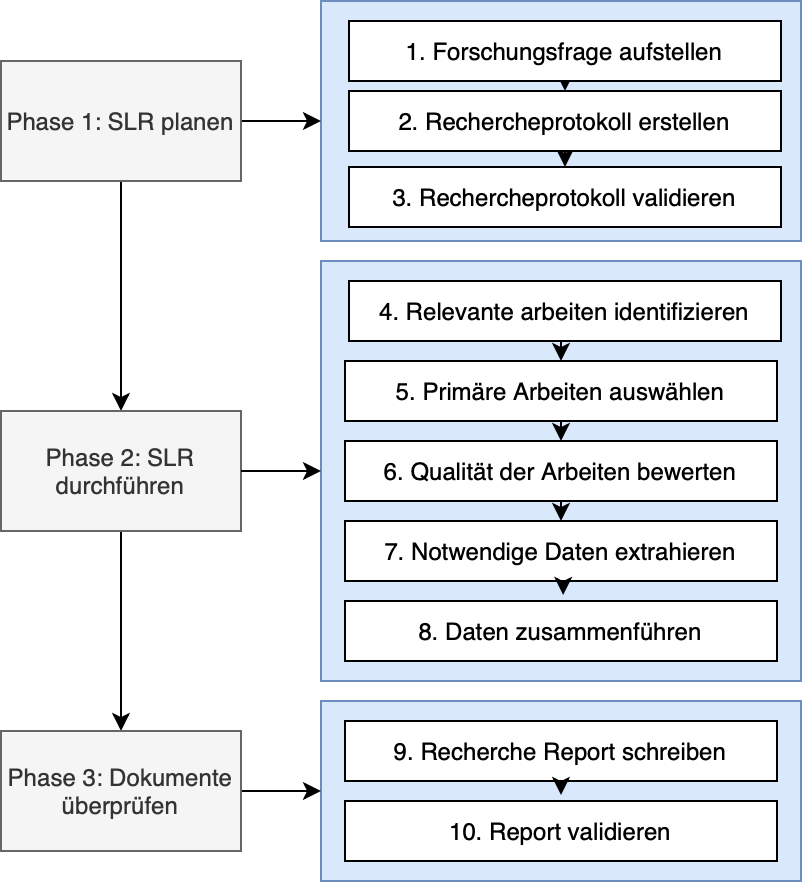
\includegraphics[width=0.8\textwidth]{graphics/slr_kitchenham_ablauf.png}
    \caption{Ablauf der systematischen Literaturrecherche nach Brereton et al. \cite{brereton2007lessons}}
    \label{fig:slr_kitchenham}
\end{figure}

\paragraph{Forschungsfrage}
Untersucht wird die Forschungsfrage: Wie können Low-Code Entwicklungsansätze 
effektiv in die Konzeption und Entwicklung von Quantencomputing-Anwendungen 
integriert werden, unter besonderer Berücksichtigung von Model-Driven 
Engineering (MDE) und Open-Source-Prinzipien?

\paragraph{Suchstrategie und Datenbanken}
In den Suchmaschinen \textit{Google Scholar}, \textit{IEEE Xplore} und \textit{ACM Digital Library} 
wird gesucht. Die Auswahl der Suchbegriffe wird strategisch vorgenommen, um die Breite und Tiefe der beiden 
Hauptthemenbereiche abzudecken. 

Die Suchbegriffe der ersten Iteration sind
\begin{itemize}
    \item \textit{Low-Code Development} 
    \item \textit{Quantum Computing}
    \item \textit{Model-Driven Engineering}
    \item \textit{Open Source}
\end{itemize} 

Um die Schnittstellen zwischen Low-Code-Plattformen und Quantencomputing genauer zu untersuchen, 
wurden die Suchbegriffe in verschiedenen Kombinationen verwendet, wobei Boolesche Operatoren wie 
AND und OR zum Einsatz kommen, um die Suche zu verfeinern und zu spezifizieren.

Die Studien müssen frühestens ab dem Jahr 2014 veröffentlicht worden sein. Dies ist insbeondere in 
Hinsicht darauf wichtig, ob das entsprechendes Tool noch aktiv gewartet wird. 
Weiterhin ist die Aktualität der Studien wichtig, da sich die Technologien und Frameworks 
im Bereich Low-Code-Entwicklung und Quantencomputing schnell weiterentwickeln.

Es werden nur Studien in englischer oder deutscher Sprache berücksichtigt, die Peer-Review-Verfahren 
durchlaufen haben. Insbesondere als relevant werden Papers erachtet, die Low-Code-Plattformen 
in Open-Source Lizensierungen behandeln. Dies vereinfacht die Verwendbarkeit für 
die spätere pilothafte Umsetzung eines Low-Code Tools für Quantencomputing-Anwendungen.

Durch die Anwendung dieser 
methodischen und strukturierten Vorgehensweise wird eine solide Basis für die Erforschung 
und Analyse der Konzeption und Entwicklung von Low-Code-Frameworks für 
Quantencomputing-Anwendungen geschaffen.

\paragraph{ResearchRabbit}
In dieser Arbeit wird ResearchRabbit als ergänzendes Tool zur systematischen Literaturrecherche eingesetzt. 
ResearchRabbit ist ein Softwaretool, das entwickelt wurde, um Arbeiten aus Forschungsgebieten als Graph darzustellen 
und relevante Verbindungen zwischen wissenschaftlichen Publikationen auf Basis von Zitierungen und thematischen 
Ähnlichkeiten zu visualisieren.\cite{cole2023researchrabbit} Nutzer des Tools geben spezifische Suchbegriffe ein, woraufhin ResearchRabbit eine 
interaktive Map generiert. Diese Maps bieten eine visuelle Darstellung, die es ermöglicht, 
zentrale Arbeiten und bisher weniger beachtete Verbindungen schnell zu identifizieren.

Die Anwendung von ResearchRabbit in der systematischen Literaturrecherche bietet erhebliche Vorteile. Erstens 
steigert das Tool die Effizienz des Rechercheprozesses, indem es durch die Visualisierung von Forschungsnetzwerken 
relevante Studien schneller erkennbar macht, was den Zeitaufwand für das erste Screening reduziert. Zweitens 
erweitert ResearchRabbit die Möglichkeit, wichtige Arbeiten zu entdecken, die in traditionellen Datenbankensuchen 
möglicherweise übersehen werden würden. Dies geschieht insbesondere durch die Aufdeckung von Querverbindungen 
zwischen verschiedenen Forschungsgebieten. Darüber hinaus ermöglicht die Analyse von Netzwerkbeziehungen 
tiefere Einblicke in die Einflussnahme und den thematischen Kontext von Schlüsselpublikationen, was zu einem 
besseren Verständnis des Forschungsstandes beiträgt. Schließlich erlaubt das Tool, aktuelle Forschungsentwicklungen 
zu verfolgen und die Literaturrecherche regelmäßig mit neuen relevanten Publikationen zu aktualisieren.

Die Entscheidung, ResearchRabbit einzusetzen, basiert auf der Notwendigkeit, eine umfangreiche und 
dynamische Forschungslandschaft effektiv zu navigieren. In sich schnell weiterentwickelnden und interdisziplinären 
Feldern wie Low-Code Development und Quantum Computing bietet ResearchRabbit einen signifikanten Mehrwert, 
indem es komplexe Informationsstrukturen zugänglich und handhabbar macht. Durch die Integration dieses Tools 
in die systematische Literaturrecherche wird nicht nur die Effizienz des Prozesses verbessert, sondern auch 
die Qualität und Tiefe der Forschungsergebnisse erhöht.

\section{Durchführung der Literaturrecherche}
Basierend auf den im vorherigen Abschnitt festgelegten Kriterien wird die systematische Literaturrecherche (SLR) 
durchgeführt. Im Folgenden werden die einzelnen Schritte der Recherche detailliert dokumentiert und die Ergebnisse 
visualisiert. Dies umfasst die spezifischen Suchanfragen in den ausgewählten wissenschaftlichen Datenbanken, die 
angewandten Suchlimits sowie die quantitativen Ergebnisse der Suchvorgänge. Durch diese detaillierte Dokumentation 
wird die Nachvollziehbarkeit und Reproduzierbarkeit der Forschung sichergestellt, während die quantitativen 
Ergebnisse eine fundierte Basis für die weitere Analyse bieten.

In der Grafik \ref{fig:search_process} ist der Ablauf der Suche nach Publikationen innerhalb der 
systematischen Literaturrecherche dargestellt. Insbesondere wird hier nochmal erwähnt, dass beim Schritt des 
Snowballings das Tool ResearchRabbit eingesetzt wird, um die Suche zu unterstützen. 

% include graphics/ablauf_der_suche.png
\begin{figure}[h!]
    \centering
    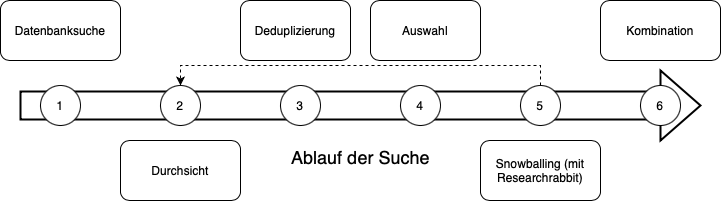
\includegraphics[width=1\textwidth]{graphics/ablauf_der_suche.png}
    \caption{Ablauf der systematischen Literaturrecherche}
    \label{fig:search_process}
\end{figure}


% \begin{itemize}
%     \item Suchprozess
%         \begin{itemize}
%             \item Durchführung der Suche in den ausgewählten Datenbanken
%                 \begin{itemize}
%                     \item Eingabe der Suchbegriffe und Kombinationen
%                     \item Anwendung von Booleschen Operatoren zur Verfeinerung
%                     \item Speichern der Suchergebnisse
%                 \end{itemize}
%             \item Dokumentation des Suchprotokolls
%                 \begin{itemize}
%                     \item Aufzeichnung der Suchbegriffe und Suchstrategien
%                     \item Festhalten der Suchergebnisse und deren Anzahl
%                     \item Datum der Suche und verwendete Datenbanken
%                 \end{itemize}
%         \end{itemize}
%     \item Screening und Auswahl der Literatur
%         \begin{itemize}
%             \item Entfernung von Duplikaten
%                 \begin{itemize}
%                     \item Identifikation und Entfernung von doppelten Einträgen
%                 \end{itemize}
%             \item Bewertung von Titeln und Abstracts
%                 \begin{itemize}
%                     \item Anwendung der Einschluss- und Ausschlusskriterien
%                     \item Erstes Screening basierend auf Titeln und Abstracts
%                     \item Dokumentation der Gründe für Ausschlüsse
%                 \end{itemize}
%             \item Volltext-Analyse
%                 \begin{itemize}
%                     \item Beschaffung der Volltexte relevanter Studien
%                     \item Detaillierte Bewertung und Anwendung der Kriterien
%                     \item Dokumentation der Gründe für endgültige Einschluss- oder Ausschlussentscheidungen
%                 \end{itemize}
%         \end{itemize}
%     \item Qualitätsbewertung der Studien
%         \begin{itemize}
%             \item Festlegung der Bewertungskriterien
%                 \begin{itemize}
%                     \item Methodische Qualität
%                     \item Validität und Verlässlichkeit der Ergebnisse
%                     \item Relevanz zur Forschungsfrage
%                 \end{itemize}
%             \item Durchführung der Qualitätsbewertung
%                 \begin{itemize}
%                     \item Anwendung der Kriterien auf die ausgewählten Studien
%                     \item Dokumentation der Bewertungsergebnisse
%                     \item Berücksichtigung der Qualität bei der Synthese der Ergebnisse
%                 \end{itemize}
%         \end{itemize}
% \end{itemize}

Um einen ersten Überblick über die Publikationen zu gewinnen wird initial die folgende Suchanfrage in den Datenbanken verwendet:

\begin{quote}
    Suchanfrage 1 (Stand: 12.07.2024):

    (''Low-Code Development'' OR ''Quantum Computing'' OR ''Model-Driven Engineering'' OR ''Open Source'')

    Erscheinungsdatum der Publikationen: 2014 - 2024
\end{quote}

\begin{table}[h!]
    \centering
    \caption{Anzahl der Suchergebnisse für Suchanfrage 1}
    \label{tab:search_1_results}
    \begin{tabular}{|l|c|}
    \hline
    \textbf{Datenbank} & \textbf{Anzahl der Ergebnisse} \\ \hline
    Google Scholar & 17.800 \\ \hline
    IEEE Xplore & 62.421 \\ \hline
    ACM Digital Library & 79.035 \\ \hline
    \end{tabular}
\end{table}
    
Diese Suchanfrage lieferte die in \ref{tab:search_1_results} dargestellten Ergebnisse. Dies 
zeigt die große Bandbreite und Relevanz der Themenfelder. 
Um hier einen Überblick zu gewinnen, wie die Verteilung der Publikationen zu den jeweiligen Konzepten ausfällt, 
wird eine Analyse der Anzahl der Publikationen pro Jahr, und Konzept, also MDE oder Low-Code vorgenommen.

Deren Ergebnisse sind in den folgenden Grafiken dargestellt:

\begin{figure}[h!]
    \centering
    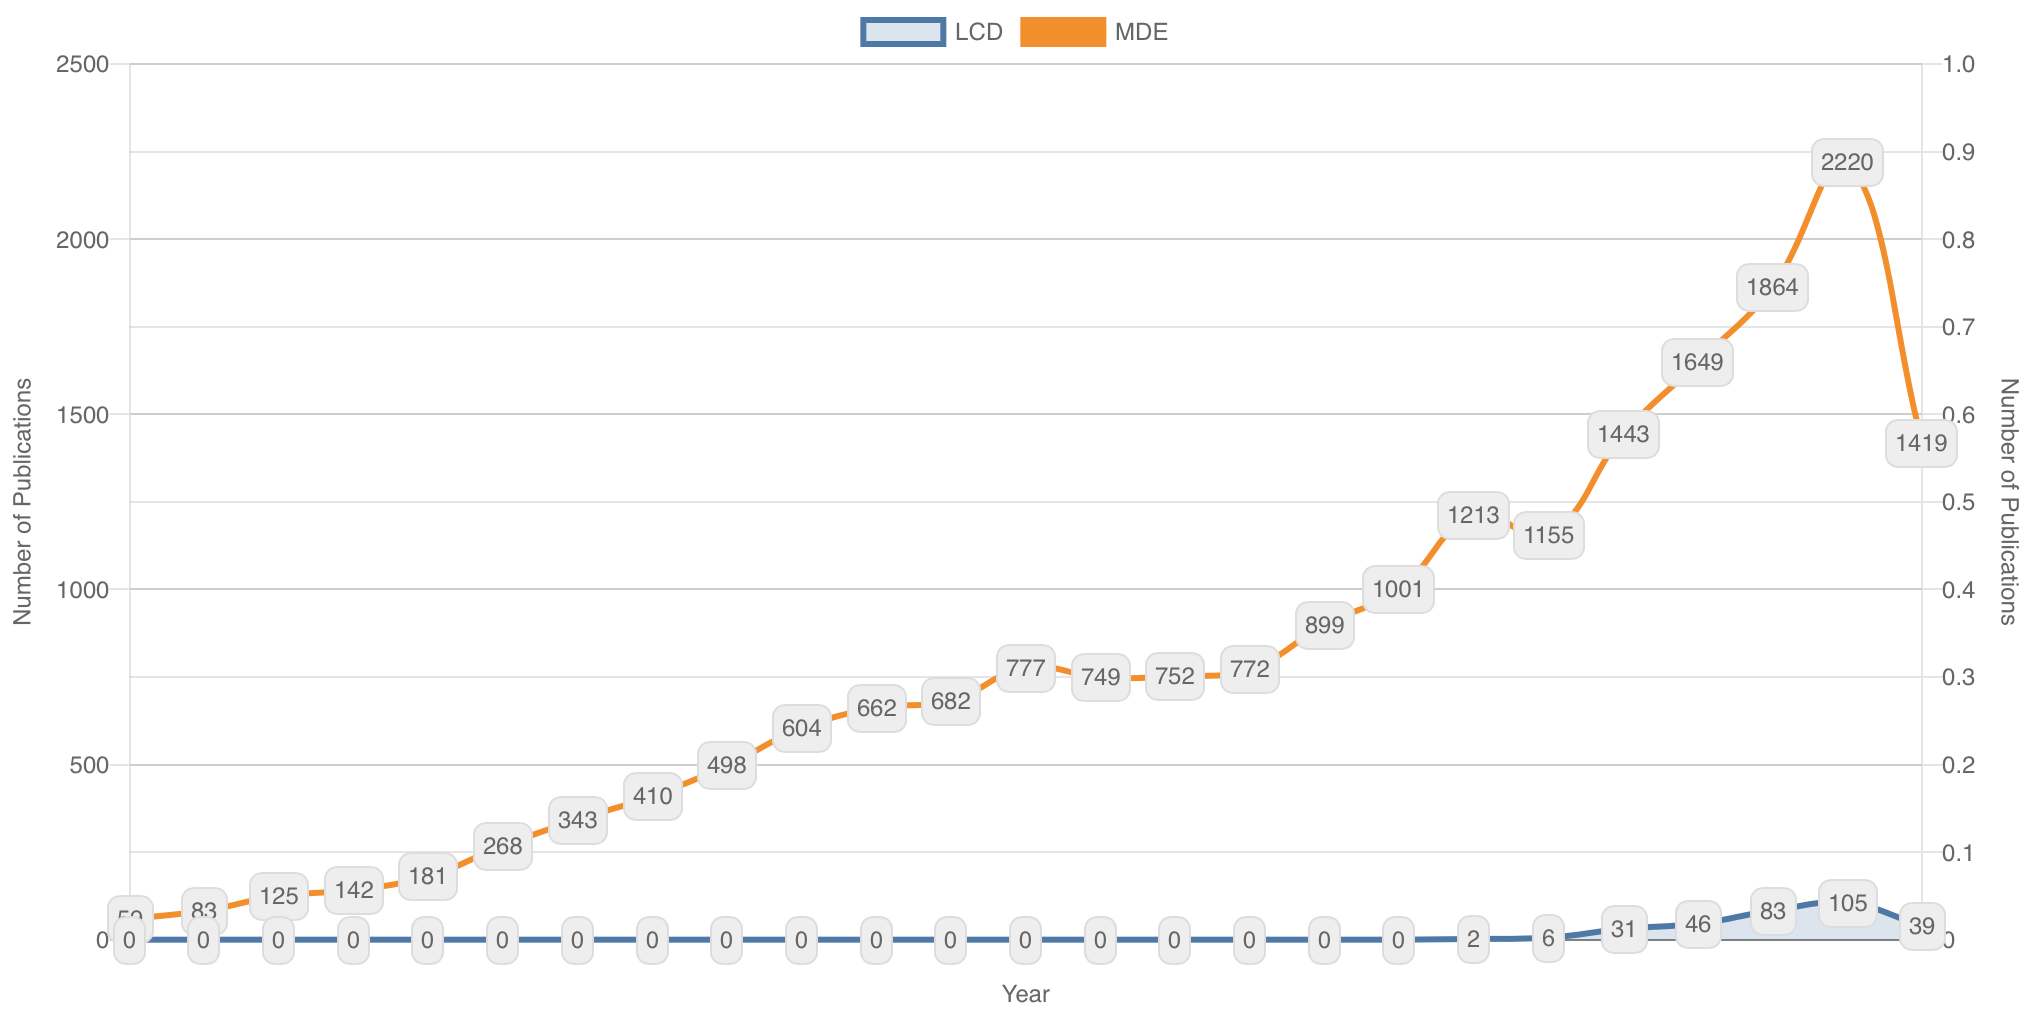
\includegraphics[width=1\textwidth]{graphics/lcd_and_mde_publications_over_years.png}
    \caption{Anzahl der Publikationen zu MDE und LCD pro Jahr}
    \label{fig:publications_mde_and_lcd_per_year}
\end{figure}

\begin{figure}[h!]
    \centering
    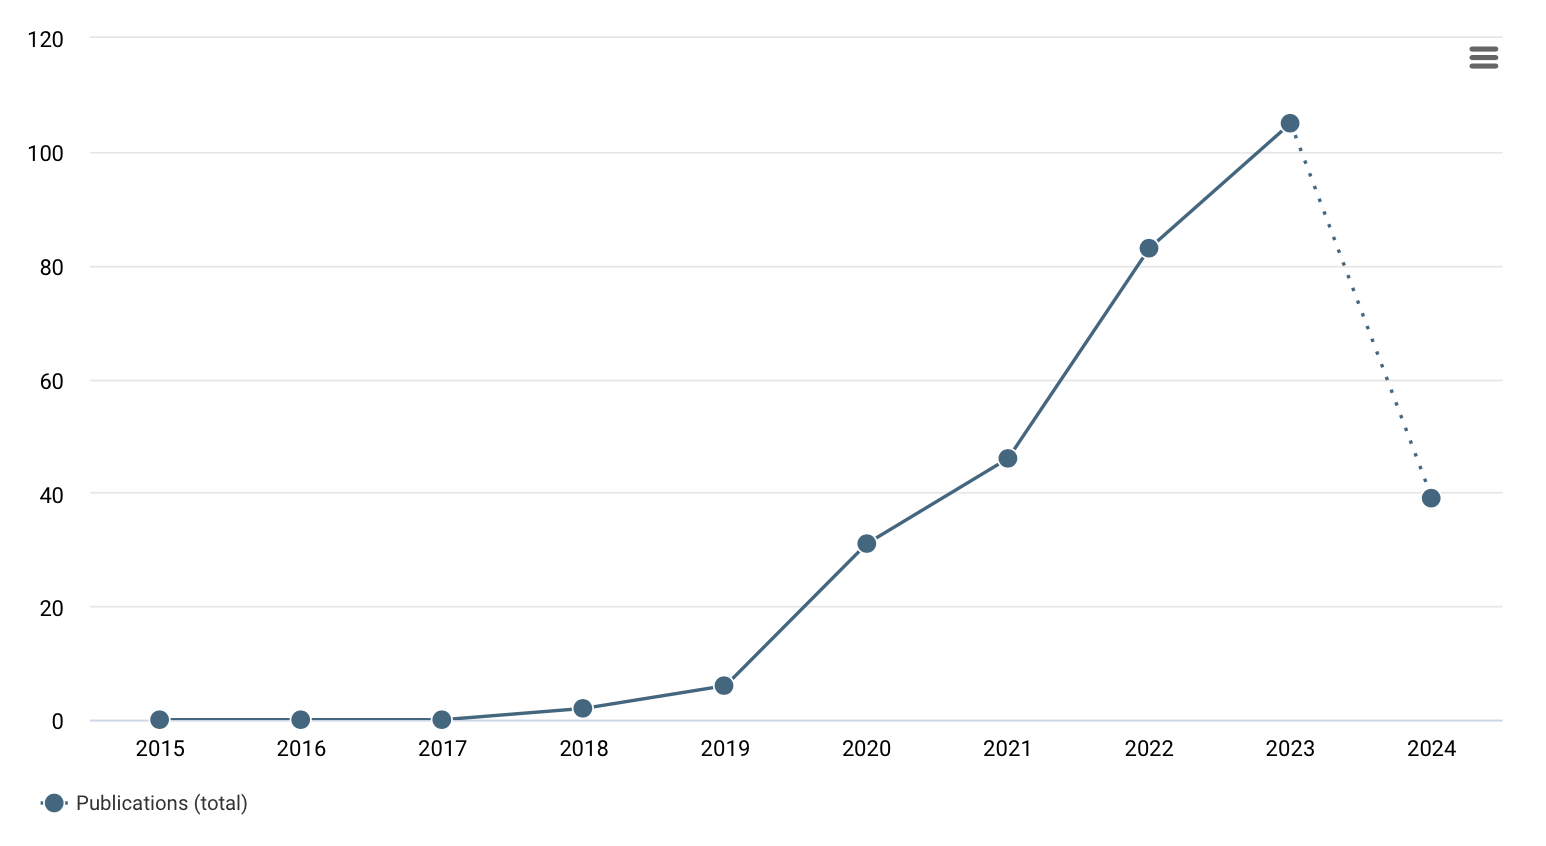
\includegraphics[width=1\textwidth]{graphics/lcd_publications_over_years.png}
    \caption{Anzahl der Publikationen LCD pro Jahr}
    \label{fig:publications_lcd_per_year}
\end{figure}

\begin{figure}[h!]
    \centering
    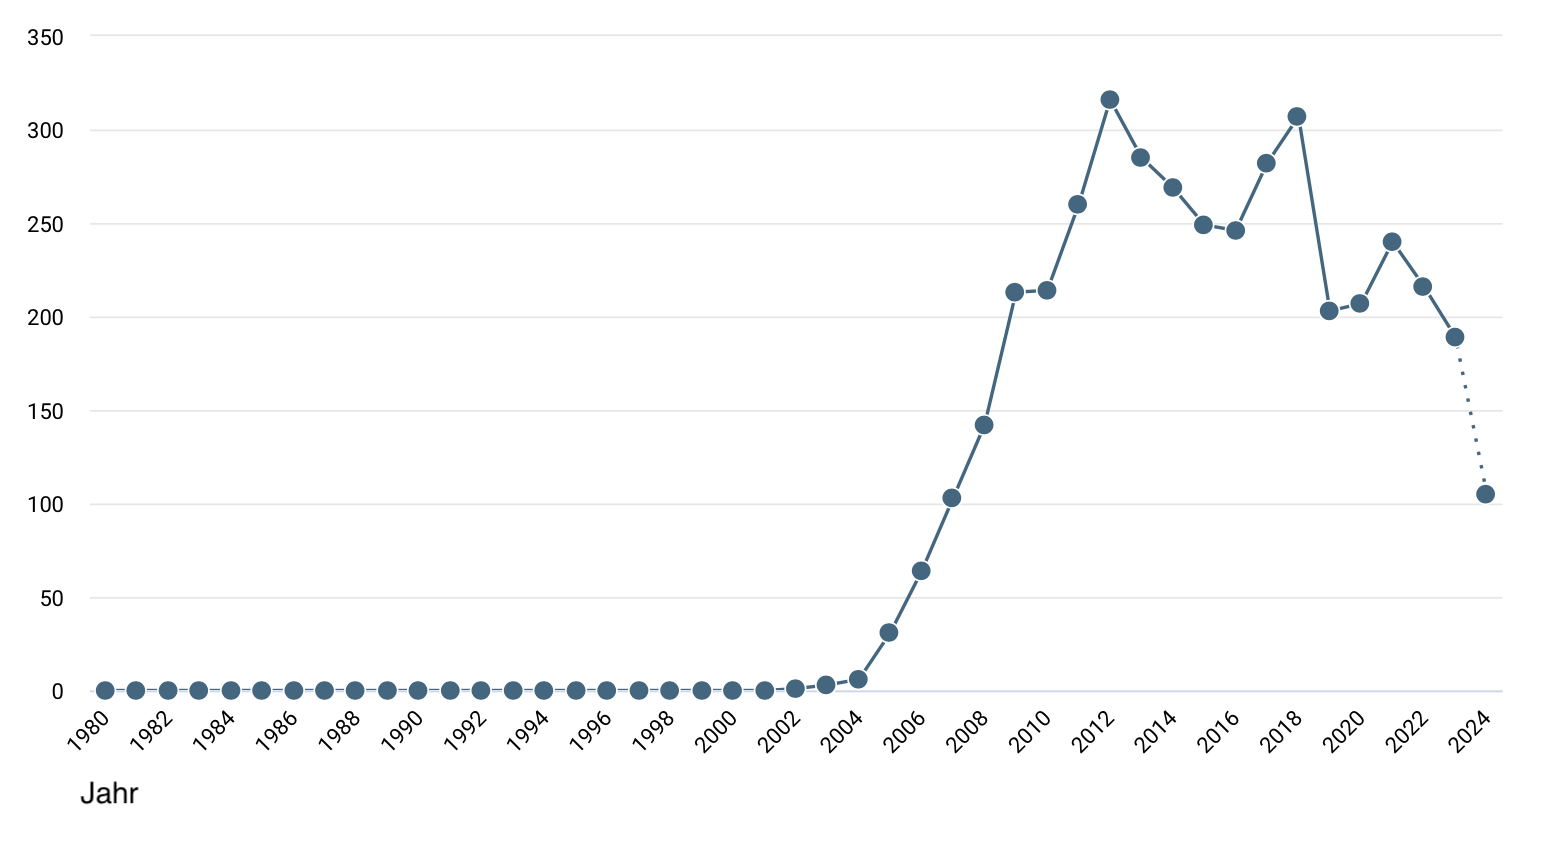
\includegraphics[width=1\textwidth]{graphics/mde_publications_over_years.png}
    \caption{Anzahl der Publikationen zu MDE pro Jahr}
    \label{fig:publications_mde_per_year}
\end{figure}

Es fällt auf, dass die Anzahl der Publikationen zu Low-Code-Entwicklung erstens insgesamt deutlich niedriger ausfällt 
als die Anzahl der Publikationen zu Model-Driven Engineering. Zweitens ist bezüglich des Erscheinungsjahres festzustellen 
das in Publikation Low-Code-Entwicklung ein deutlich jüngeres Forschungsthema ist.

Da die Anzahl der Ergebnisse zu groß ist um effektiv bearbeitet zu werden, wird die Suche 
weiter verfeinert. Weiterhin fällt beim ersten Screening auf, dass viele Ergebnisse nicht die 
gewünschte Schnittmenge aus Low-Code-Entwicklung und Quantencomputing abdecken, sondern 
nur eines der beiden Themenfelder behandeln. Um also die Relevanz der Ergebnisse zu erhöhen, 
werden spezifischere Suchanfragen formuliert. 

In einer zweiten Iteration der Suche wurde daher die folgende Suchanfrage verwendet:

\begin{quote}
    Suchanfrage 2 (Stand: 14.07.2024):

    (''Low Code Platform'' OR ''Low Code Development'' OR ''Low-Code Development'' OR ''Model-Driven Engineering'') AND (''Quantum Computing'')

    Erscheinungsdatum der Publikationen: 2014 - 2024
\end{quote}

\begin{table}[h!]
    \centering
    \caption{Anzahl der Suchergebnisse für Suchanfrage 2}
    \label{tab:search_2_results}
    \begin{tabular}{|l|c|}
    \hline
    \textbf{Datenbank} & \textbf{Anzahl der Ergebnisse} \\ \hline
    Google Scholar & 176 \\ \hline
    IEEE Xplore & 3 \\ \hline
    ACM Digital Library & 30 \\ \hline
    \end{tabular}
\end{table}

Die Ergebnisse der zweiten Suchanfrage sind in Tabelle \ref{tab:search_2_results} dargestellt. Bzgl. der Erscheinungsjahre fällt auf, dass in 
IEEE Xplore die drei Publikationen zwischen 2021 und 2023 erschienen. in der ACM Digital Library sind die Publikationen zwischen 2021 und 2024 erschienen. 
Lediglich die Google Scholar Suche ergab Publikationen, die bis ins Jahr 2014 als Untergrenze der gewünschten Filterung zurückreichen. 

Da die Anzahl der Ergebnisse nun sinnvoller ist, wird mit der Durchsicht der Titel und Abstracts fortgefahren. 
Begonnen wird mit den drei Ergebnissen aus IEEE Xplore. Durchsicht der Abstracts ergibt, dass die Publikationen 
alle drei relevant sind, da sie sich inhaltlich in der Schnittmenge aus MDE und Quantencomputing befinden. 
Um für die Datenbank IEEE Xplore den Schritt der Auswahl vorwegzugreifen, werden die drei Publikationen 
direkt in die engere Auswahl übernommen. 

Als nächsten werden die Ergebnisse der ACM Digital Library ebenfalls durchgesehen. Dabei werden beim Schritt der Auswahl notwendigerweise die 
Ergebnisse der ACM Digital Library gezielt gefiltert, um die Relevanz und Qualität der eingeschlossenen Studien sicherzustellen. 
Proceedings wurden dabei bewusst nicht in die Auswahl einbezogen. Der Grund dafür ist, dass Proceedings häufig eine 
Vielzahl von Kurzbeiträgen enthalten, die nicht denselben rigorosen Peer-Review-Prozess durchlaufen wie Journal-Artikel 
und oft eine geringere wissenschaftliche Tiefe aufweisen. Dies kann die Validität und Verlässlichkeit der 
Forschungsergebnisse beeinträchtigen. Zudem sind Proceedings meist vorläufige Ergebnisse, die 
später in detaillierteren Journal-Artikeln veröffentlicht werden. Von den initialen 30 Ergebnissen 
in der ACM Digital Library erfüllten lediglich 4 die AuswahlkriterienDurch diese Vorgehensweise wurde 
sichergestellt, dass nur qualitativ hochwertige und relevante Studien in die Analyse einbezogen wurden.

Weiterhin wurden Publikationen ausgeschlossen, deren Titel oder Abstract darauf schließen ließen, dass sie thematisch 
nicht relevant sind. Dieser Ausschluss erfolgte, um die Fokussierung auf Studien zu gewährleisten, die direkt mit 
Low-Code-Entwicklungsansätzen in Quantencomputing-Anwendungen verbunden sind. Diese strenge Selektion ist entscheidend, um 
sicherzustellen, dass die verbleibenden Studien tatsächlich die Forschungsfrage adressieren und qualitative Erkenntnisse liefern können. 

Durchsicht der 176 Ergebnisse aus Google Scholar ergab, dass 20 Publikationen die Kriterien für die engere Auswahl erfüllen. 

Für den Schritt der Deduplizierung wurden die Ergebnisse aus den drei Datenbanken zusammengeführt. 
So ergeben sich ohne Duplikate insgesamt 25 Publikationen, die für die weitere Analyse in Betracht gezogen werden. 

Bevor durch Snowballing weitere möglicherweise relevante Publikationen gesucht werden und die Volltexte der Publikationen analysiert werden, 
wird eine dritte Suchanfrage formuliert. Diese zielt darauf ab, durch eine noch feinere Fomulierung der Anfrage weitere bisher nicht gefundene 
Ergebnisse zu identifizieren. 

\begin{quote}
    Suchanfrage 3 (Stand: 16.07.2024):

    (intitle:''low-code'' quantum computing)

    Erscheinungsdatum der Publikationen: 2014 - 2024
\end{quote}

Hierfür ergibt sich die in Tabelle \ref{tab:search_3_results} dargestellte Anzahl an Ergebnissen. 

\begin{table}[h!]
    \centering
    \caption{Anzahl der Suchergebnisse für Suchanfrage 3}
    \label{tab:search_3_results}
    \begin{tabular}{|l|c|}
    \hline
    \textbf{Datenbank} & \textbf{Anzahl der Ergebnisse} \\ \hline
    Google Scholar & 26 \\ \hline
    IEEE Xplore & 1 \\ \hline
    ACM Digital Library & 8 \\ \hline
    \end{tabular}
\end{table}

Erneut ist die Anzahl an Suchergebnissen geringer geworden. Durchsicht der neuen Ergebnisse ergibt, dass zwar aus Google Scholar 
keine weiteren Publikationen in die engere Auswahl übernommen werden, jedoch aus der ACM Digital Library 7 sowie aus IEEE Xplore 1 Publikation. 
Insgesamt ergibt sich somit eine Anzahl von 33 unterschiedlichen Publikationen, die für die weitere Analyse in Betracht gezogen werden. 

Mit den nun identifizierten Publikationen wird der Schritt des Snowballings durchgeführt. Hierbei wird ResearchRabbit eingesetzt, um 
weitere Publikationen zu identifizieren, die inhaltlich mit den bereits identifizierten Publikationen in Verbindung stehen und somit 
potenziell relevant sind. Das Tool zeigt dabei die Verbindungen zwischen den Publikationen an und ermöglicht es, die Netzwerke 
zu älteren und neueren Publikationen zu visualisieren. Es ergeben sich 21 ältere Publikationen, die mit den bereits identifizierten 33 
Publikationen in Verbindung stehen. Dazu kommen 6 neuere die auf die bereits identifizierten Publikationen verweisen. 

Für diese wird nun ebenfalls der Titel und Abstract durchgesehen, um zu entscheiden, ob sie in die engere Auswahl übernommen werden. 
Insgesamt lassen sich so 13 weitere Publikationen identifizieren, die für die weitere Analyse in Betracht gezogen werden, was nun nach 
dem Schritt der Kombination zu 46 Publikationen führt. 

\section{Ergebnisse}
\begin{itemize}
    \item Übersicht der identifizierten Studien
        \begin{itemize}
            \item Anzahl der gefundenen Studien nach dem Screening
            \item Verteilung der Studien nach Jahr, Autor und Quelle
            \item Kategorisierung nach Themenbereichen (z.B. Low-Code Development, Quantum Computing, MDE, Open Source)
        \end{itemize}
    \item Synthese der Ergebnisse
        \begin{itemize}
            \item Zusammenfassung der Hauptbefunde
                \begin{itemize}
                    \item Gemeinsame Trends und Muster in den identifizierten Studien
                    \item Unterschiede und Besonderheiten in den Ansätzen
                \end{itemize}
            \item Integration der Erkenntnisse
                \begin{itemize}
                    \item Wie die Ergebnisse zur Beantwortung der Forschungsfragen beitragen
                    \item Bedeutung der Ergebnisse im Kontext der Entwicklung eines Low-Code-Frameworks für Quantencomputing
                \end{itemize}
            \item Identifikation von Forschungslücken
                \begin{itemize}
                    \item Bereiche mit wenig oder keiner Forschung
                    \item Vorschläge für zukünftige Forschungsrichtungen
                \end{itemize}
        \end{itemize}
    \item Bewertung der Ergebnisse
        \begin{itemize}
            \item Kritische Analyse der Qualität und Relevanz der gefundenen Studien
                \begin{itemize}
                    \item Stärken und Schwächen der Studien
                    \item Zuverlässigkeit und Validität der Ergebnisse
                \end{itemize}
            \item Schlussfolgerungen basierend auf der Synthese
                \begin{itemize}
                    \item Wichtige Erkenntnisse und ihre Implikationen
                    \item Empfehlungen für die Entwicklung des Low-Code-Frameworks
                \end{itemize}
        \end{itemize}
\end{itemize}

\subsection*{Anhang 1: Übersicht der Publikationen}

\setcounter{table}{0}
\renewcommand{\thetable}{A\arabic{table}}

% create a longtable to list all publications
\begin{longtable}{|m{0.8cm}|m{4.4cm}|m{3cm}|m{0.8cm}|m{4cm}|}
    \caption{Übersicht der Publikationen} 
    \label{tab:publikationen} \\
    \hline
    \textbf{ID} & \textbf{Titel} & \textbf{Autoren} & \textbf{Jahr} & \textbf{Themengebiet} \\
    \hline
    \endhead
    P01 & In Search of the Essence of Low-Code: An Exploratory Study of Seven Development Platforms & Alexander C. Bock, Ulrich Frank~\cite{Bock_2021_essence} & 2021 & Low-Code,  \\ \hline
    P02 & What about the usability in low-code platforms? A systematic literature review & Daniel Pinho et al.~\cite{Pinho_2022} & 2022 & Low-Code,  \\ \hline
    P03 & Low-Code Development Platforms - A Literature Review & Niculin Prinz et al.~\cite{Prinz_2021} & 2021 & Low-Code,  \\ \hline
    P04 & Supporting the understanding and comparison of low-code development platforms & Apurvanand Sahay et al.~\cite{Sahay_2020} & 2020 & Low-Code,  \\ \hline
    P05 & Building BESSER: an open-source low-code platform & Iván Alfonso et al.~\cite{alfonso2024building} & 2024 & Low-Code,  \\ \hline
    P06 & AI for Low-Code for AI & Nikitha Rao et al.~\cite{rao2024} & 2024 & Low-Code,  \\ \hline
    P07 & Challenges \& opportunities in low-code testing & Faezeh Khorram et al.~\cite{Khorram_2020} & 2020 & Low-Code,  \\ \hline
    P08 & Low-Code Is Often High-Code, So We Must Design Low-Code Platforms to Enable Proper Software Engineering & Timothy C. Lethbridge~\cite{lethbridge2021low} & 2021 & Low-Code,  \\ \hline
    P09 & Low-Code, No-Code, What's Under the Hood? & George Hurlburt~\cite{Hurlburt_2021} & 2021 & Low-Code,  \\ \hline
    P10 & Drivers and Inhibitors of Low Code Development Platform Adoption & Sebastian Kass et al.~\cite{Kass_2022} & 2022 & Low-Code,  \\ \hline
    P11 & A Low-Code Approach for Simulation-Based Analysis of Process Collaborations & Paolo Bocciarelli, Andrea D'Ambrogio~\cite{Bocciarelli_2023} & 2023 & Low-Code, Model-Driven Engineering,  \\ \hline
    P12 & Developer discussion topics on the adoption and barriers of low code software development platforms & Md Abdullah Al Alamin et al.~\cite{Alamin_2022} & 2022 & Low-Code, Model-Driven Engineering,  \\ \hline
    P13 & Quantumoonlight: A Low-Code Platform to Experiment with Quantum Machine Learning & Francesco Amato et al.~\cite{amato2023quantumoonlight} & 2023 & Low-Code, Quantum Computing,  \\ \hline
    P14 & Towards a Quantum Software Modeling Language & Carlos A. Pérez-Delgado et al.~\cite{Perez-Delgado_2020} & 2020 & Low-Code, Quantum Computing, Model-Driven Engineering,  \\ \hline
    P15 & Model-Driven Quantum Federated Learning (QFL) & Armin Moin et al.~\cite{Moin_2023} & 2023 & Low-Code, Quantum Computing, Model-Driven Engineering,  \\ \hline
    P16 & Towards Model-Driven Quantum Software Engineering & Felix Gemeinhardt et al.~\cite{gemeinhardt_2021} & 2021 & Low-Code, Quantum Computing, Model-Driven Engineering,  \\ \hline
    P17 & A Model-Driven Framework for Composition-Based Quantum Circuit Design & Felix Gemeinhardt et al.~\cite{Gemeinhardt_2018} & 2018 & Low-Code, Quantum Computing, Model-Driven Engineering,  \\ \hline
    P18 & A Reference Architecture for Quantum Computing as a Service & Aakash Ahmad et al.~\cite{Ahmad_2023} & 2023 & Low-Code, Quantum Computing, Model-Driven Engineering,  \\ \hline
    P19 & Design of classical-quantum systems with UML & Ricardo Pérez-Castillo et al.~\cite{perez2022design} & 2022 & Low-Code, Quantum Computing, Model-Driven Engineering,  \\ \hline
    P20 & Integrating Quantum Computing into Workflow Modeling and Execution & Benjamin Weder et al.~\cite{Weder_2020} & 2020 & Low-Code, Quantum Computing, Model-Driven Engineering,  \\ \hline
    P21 & Towards Quantum-algorithms-as-a-service & Manuel De Stefano et al.~\cite{Stefano_2022} & 2022 & Low-Code, Quantum Computing, Model-Driven Engineering,  \\ \hline
    P22 & Survey and classification of model transformation tools & Nafıseh Kahani et al.~\cite{Kahani_2019} & 2019 & Model-Driven Engineering,  \\ \hline
    P23 & Quantum Software Development with Classiq & Nir Minerbi~\cite{minerbi2022quantum} & 2022 & Quantum Computing,  \\ \hline
    P24 & Challenges of Quantum Software Engineering for the Next Decade: The Road Ahead & J. M. Murillo et al.~\cite{murillo2024challenges} & 2024 & Quantum Computing,  \\ \hline
    P25 & Software Architecture for Quantum Computing Systems - A Systematic Review & Arif  Ali Khan et al.~\cite{Khan_2022} & 2022 & Quantum Computing,  \\ \hline
    P26 & On the Definition of Quantum Programming Modules & Pedro Sánchez, Diego Alonso~\cite{Sanchez_2021} & 2021 & Quantum Computing,  \\ \hline
    P27 & Generation of Classical-Quantum Code from UML models & Ricardo Pérez-Castillo et al.~\cite{Perez-Castillo_2023} & 2023 & Quantum Computing, Model-Driven Engineering,  \\ \hline
    P28 & Model-Driven Optimization for Quantum Program Synthesis with MOMoT & Felix Gemeinhardt et al.~\cite{Gemeinhardt_2023} & 2023 & Quantum Computing, Model-Driven Engineering,  \\ \hline
    P29 & Reverse Engineering of OpenQASM3 Quantum Programs to KDM Models & Luis Jiménez-Navajas et al.~\cite{Jimenez-Navajas_2023} & 2023 & Quantum Computing, Model-Driven Engineering,  \\ \hline
    P30 & A Graph-Based Approach for Modelling Quantum Circuits & Diego Alonso et al.~\cite{alonso2023graph} & 2023 & Quantum Computing, Model-Driven Engineering,  \\ \hline
    P31 & MDE4QAI: Towards Model-Driven Engineering for Quantum Artificial Intelligence & Moin, Armin et al.~\cite{Moin_2021} & 2021 & Quantum Computing, Model-Driven Engineering,  \\ \hline
    P32 & Engineering the development of quantum programs: Application to the Boolean satisfiability problem & Diego Alonso et al.~\cite{Alonso_2022} & 2022 & Quantum Computing, Model-Driven Engineering,  \\ \hline
    P33 & Model-Driven Engineering for Quantum Programming: A Case Study on Ground State Energy Calculation & Furkan Polat et al.~\cite{polat2024model} & 2024 & Quantum Computing, Model-Driven Engineering,  \\ \hline
    P34 & Kdm to uml model transformation for quantum software modernization & Luis Jiménez-Navajas et al.~\cite{Jimenez-Navajas_2021} & 2021 & Quantum Computing, Model-Driven Engineering,  \\ \hline
    P35 & Modeling Quantum programs: challenges, initial results, and research directions & Shaukat Ali et al.~\cite{Ali_2020} & 2020 & Quantum Computing, Model-Driven Engineering,  \\ \hline
    P36 & Transforming Quantum Programs in Kdm to Quantum Design Models in Uml & Luis Jiménez-Navajas et al.~\cite{Jimenez-Navajas_2022} & 2022 & Quantum Computing, Model-Driven Engineering,  \\ \hline
    P37 & Toward a Quantum Software Engineering & Mario Piattini et al.~\cite{Piattini_2021} & 2021 & Quantum Computing, Model-Driven Engineering,  \\ \hline
    P38 & Software architecture for quantum computing systems - A systematic review & Arif Ali Khan et al.~\cite{khan2023software} & 2023 & Quantum Computing, Model-Driven Engineering,  \\ \hline
    P39 & Classical to Quantum Software Migration Journey Begins: A Conceptual Readiness Model & Muhammad Azeem Akbar et al.~\cite{Akbar_2022} & 2022 & Quantum Computing, Model-Driven Engineering,  \\ \hline
    P40 & Modelling Quantum Circuits with UML & Ricardo Pérez‐Castillo et al.~\cite{Perez-Castillo_2021} & 2021 & Quantum Computing, Model-Driven Engineering,  \\ \hline
    P41 & MDE4QAI: Towards Model-Driven Engineering for Quantum Artificial Intelligence & Armin Moin et al.~\cite{Moin_2021} & 2021 & Quantum Computing, Model-Driven Engineering,  \\ \hline
\end{longtable}

